% ísticos que baseiam-se na %--------------------------------------------------------------------------------------
% Este arquivo contém a sua metodologia
%--------------------------------------------------------------------------------------
\chapter{Materiais e Métodos} \label{ch:MateriaisMétodos} %Uma label é como você referencia uma seção no texto com a tag \ref{}
    % Neste capítulo será apresentado como será feita a avaliação do desempenho das funções de ranqueamento na Mineração de Texto.
    Neste capítulo será apresentado como será feita a avaliação do desempenho da função de ranqueamento BM25 como atributo em Mineração de Texto.
    A metodologia proposta está ilustrada na Figura \ref{fig:diagrama-da-metodologia} e o processo é detalhado a seguir.
    
    \begin{figure}[H]
    \centering
    \caption{Metodologia proposta para avaliação de desempenho, em verde estão as variáveis mensuráveis sugeridas.}
    \begin{center}
        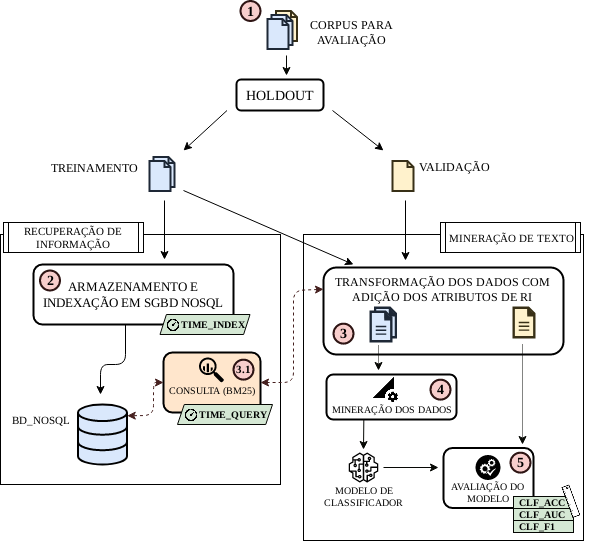
\includegraphics[width=0.8\textwidth]{img/diagrama-metodologia-v2-2.png}
    \end{center}
    \vspace{-0.5cm}
    \legend{\ABNTEXfontereduzida \textbf{Fonte:} O autor.}
    \label{fig:diagrama-da-metodologia}
\end{figure}
    
    Inicialmente é necessário selecionar os \textbf{(1) Banco de Dados para Avaliação} que servirão para efetuar as avaliações de desempenho, e, caso essas bases de dados ainda não estejam segmentados em exemplos para treinamento e exemplos para validação, será feita essa separação com o método de \textit{holdout} de $\frac{2}{3}$ para treinamento e $\frac{1}{3}$ para validação.
    
    Em seguida, o conjunto de treinamento passará pela fase de RI, aonde será feito o \textbf{(2) Armazenamento e Indexação em  SGBD NoSQL} por meio das ferramentas apresentadas na Seção  \ref{sec:Armazenamento-e-indexação}, sendo mensurado o tempo necessário para concluir essa operação em cada um dos Sistemas Gerenciadores de Banco de Dados (SGBD) NoSQL selecionados.
    
    O processo de Mineração de Texto pode ser segmentado em 7 etapas, conforme ressaltado anteriormente na Seção \ref{sec:MineraçãoTexto}.
    E, na metodologia proposta aqui, a fase de MT assume que as 3 etapas iniciais de limpeza, integração, e seleção dos dados, já foram realizadas no banco de dados de teste, assim os conjuntos divididos em treinamento e validação passarão diretamente pela etapa seguinte que é a \textbf{(3) Transformação dos dados com adição dos atributos de RI}.
    Nesta etapa serão feitas consultas ao banco de dados NoSQL que foi indexado com a utilização das funções de ranqueamento baseadas no BM25 que cada ferramente implementa, sendo mensurado o tempo para efetuar cada consulta e gerar os novos atributos sugeridos adiante na Seção \ref{sec:Atributos-de-RI-sugeridos}.
    
    O processo de Mineração dos Dados será feito por reprodução de soluções dos bancos de dados para avaliação selecionados e que possuam seus códigos fonte disponíveis, sendo então reproduzida a solução sem nenhuma alteração e então a mesma será reproduzida com os novos atributos sugeridos.
    Esse processo gerará dois modelos de classificador, o primeiro criado sem atributos de RI e o segundo com esses atributos.
    A etapa de \textbf{(4) Avaliação do Modelo} permitirá que, para cada modelo, sejam geradas métricas da literatura de MT (detalhadas logo mais na Subseção \ref{subsec:Desempenho-de-classificador}) a partir do teste com o conjunto de validação, permitindo a comparação do ganho de desempenho de classificador com/sem atributos de RI.
    % Na fase de Mineração de Texto os conjuntos de treinamento e de validação passarão pela \textbf{(3) Transformação dos dados com adição dos atributos de RI} onde 
    
    
    % Para utilização da função de ranqueamento BM25 como variável em tarefas de mineração de texto é necessário efetuar o armazenamento e a indexação dos textos do conjunto de treinamento, e para esta tarefa serão utilizadas ferramentas de armazenamento em banco de dados (não relacionais?) que fornecem implementações do BM25 para consulta, estas serão apresentadas na Seção \ref{sec:Armazenamento-e-indexação}.
    
    % Se faz necessário também definir métricas para avaliação do ganho de desempenho com as variáveis de RI, assim como elencar as bases de dados que vão servir para efetuar essa avaliação, disposto logo mais nas Seções \ref{sec:Métricas-para-avaliação-de-desempenho} e \ref{sec:Bancos-de-dados-para-avaliação}.

\section{Bancos de dados para avaliação}  \label{sec:Bancos-de-dados-para-avaliação}
    Os banco de dados de teste selecionados para avaliação são os utilizados na PanCLEF 2019 % necessário citar a PanCLEF anteriormente

    \begin{itemize}
        \item Bots and Gender Profiling PAN @ CLEF 2019
        % https://pan.webis.de/clef19/pan19-web/author-profiling.html
        \item Hyperpartisan News Detection - PAN @ SemEval 2019
        %  https://pan.webis.de/semeval19/semeval19-web/index.html
    \end{itemize}
    % Descreuioes a partir da tarefa no site
    % Definir as soluçcoes disponiveis que vou utilizar (Nao pode ter RI)

\section{Armazenamento e indexação} \label{sec:Armazenamento-e-indexação}

    Para armazenar e indexar os bancos de dados das tarefas de Mineração de Textos, e possibilitar assim o cálculo da função BM25 para cada exemplo, serão utilizadas as seguintes tecnologias que fazem implementações do BM25:
    \begin{itemize}
        \item Elasticsearch % https://www.elastic.co/guide/en/elasticsearch/reference/current/index-modules-similarity.html
        % https://www.elastic.co/pt/blog/practical-bm25-part-2-the-bm25-algorithm-and-its-variables
        \item ArangoDB
        % https://www.arangodb.com/docs/stable/aql/views-arango-search.html#bm25
        % https://www.arangodb.com/news/introducing-arangodb-3-4/
        \item Zettair
        % http://www.seg.rmit.edu.au/zettair/doc/Readme.html
        % \item Apache Spark
        % COmentado pois o Spark não implementa o BM25.
    \end{itemize}
    % Links dos sites das ferramentas como notas de rodapé.
    % Citar a versão de cada ferramenta que vai ser utilizada.
    % 
    

 
% Metodologia:

% Vão ser elencadas as tecnologias para armazenamento e indexação dos dados por meio do BM25:
% * Elasticsearch
% * APache Spark
% * ArangoDB
% * Zettair

% Os bancos de teste serão:
% * PanCLEF Hyperpartisan 2019
% https://pan.webis.de/semeval19/semeval19-web/leaderboard.html
% * A definir
% * Bots and Gender Profilin % PAN @ CLEF 2019 

\section{Atributos de RI sugeridos}  \label{sec:Atributos-de-RI-sugeridos}
    
%  Por exemplo, para a classificação binária do PANCLEF 2019 Hyperpartisan podem ser criadas as variáveis a seguir:
% * avg_0 
% * count_0
% * sum_0
% * avg_1
% * count_1
% * sum_1

% baseadas no weren (2014)


\section{Métricas para avaliação de desempenho}  \label{sec:Métricas-para-avaliação-de-desempenho}
    Será avaliado o desempenho das ferramentas utilizadas para indexação e consulta, por meio da avaliação temporal do desempenho computacional, e também o ganho de desempenho propiciado pelo uso das variáveis de RI em termos das métricas de classificadores de Mineração de Texto. % Essas métricas tem que ser citadas no referencial teórico.
    
    \subsection{Desempenho computacional das ferramentas}  \label{subsec:Desempenho-computacional}
        Para avaliar o desempenho das ferramentas de armazenamento e indexação utilizaremos duas métricas temporais:
        \begin{itemize}
            \item \textbf{TIME\_INDEX}: Tempo de execução para indexar o conjunto de treinamento de cada um dos banco de dados de teste elencados na Seção \ref{sec:Bancos-de-dados-para-teste}. Dadas as quatro diferentes ferramentas de indexação e os dois banco de dados selecionados, serão computadas 8 TIME\_INDEX para comparação;
            
            \item \textbf{TIME\_QUERY}: Tempo para consulta de cada exemplo do conjunto de teste e geração das variáveis sugeridas na Seção \ref{sec:Variáveis-de-RI-sugeridas} para o item específico. Dadas as 12 variáveis sugeridas para criação distribuídas nos dois banco de dados selecionados, e dadas as 4 ferramentas de indexação, 48 TIME\_QUERY serão computadas.  
        \end{itemize}
        
        Essas variáveis serão computadas para cada uma das 4 ferramentas selecionadas sendo executadas no mesmo sistema computacional a fim de oferecer maior confiança aos números obtidos. 
        O sistema computacional a ser utilizado para efetuar o experimento ainda não está definido, mas será especificado nos resultados.
    
% O teste de desempenho será feito comparando as ferramentas de indexação, tempo para indexar o treino de cada banco (TIME_TRN) em cada ferramenta.

% O tempo para consultar para cada linha do teste as variáveis a serem criadas (no caso de classificação binária iremos definir agregações do tipo count, sum e avg). Por exemplo, para a classificação binária do PANCLEF 2019 Hyperpartisan podem ser criadas as variáveis a seguir:
% * avg_0 
% * count_0
% * sum_0
% * avg_1
% * count_1
% * sum_1
    \subsection{Desempenho de classificador}  \label{subsec:Desempenho-de-classificador}
    O ganho de desempenho propiciado pelas variáveis de RI criadas será mensurado por métricas de desempenho de classificadores da literatura de Mineração de Dados, as mesmas da Mineração de Texto.
    Nesse estudo serão computadas as seguintes métricas:
    \begin{itemize}
        \item \textbf{CLF\_ACC}: Acurácia do classificador.
        \item \textbf{CLF\_AUC}: Área sobre a curva ROC.
        \item \textbf{CLF\_F1}: F1-Score
        \item \textbf{CLF\_PRE}: Precisão do classificador.
        \item \textbf{CLF\_REC}: Revocação do classificador.
    \end{itemize}
% Ao final será comparado o ganho de desempenho (acurácia, precisão, recall e F1-score) nas melhores soluções dos bancos definidos a partir da adição das variáveis criadas.
% Por exemplo para a PANCLEF 2019 Hyperpartisan será utilizada a solução que está disponível no github com melhor score e ela será executada novamente para conferir o resultado obtido de acurária que eles dizem e então será rodado novamente com a adição das variáveis de RI (BM25).


ADICIONAR IMAGEM DE VISÃO GERAL DA METODOLOGIA


% \subsection{Subseção de exemplo 1 - Referenciando seções} \label{subsec:subsec1}






%--------------------------------------------------------------------------------------
% Insere a seção de cronograma
% Está comentada porque só é necessária no TCC I
%--------------------------------------------------------------------------------------
% %--------------------------------------------------------------------------------------
% Insere a seção de cronograma
%--------------------------------------------------------------------------------------

\section{Cronograma} \label{sec:Cronograma}

A Tabela \ref{tab:cronograma} mostra o cronograma de atividades a serem executadas para o Trabalho de Conclusão II (TCC II), com base no calendário do período 2019.2 da UNIVASF, definido pelo Calendário Acadêmico 2019 da instituição.

\begin{table}[!thb]
	%\huge
    \centering
    \caption{Cronograma das atividades previstas para o TCC II.}
    \begin{adjustbox}{max width=\textwidth}
    \begin{tabular}{p{6.5cm}|c|c|c|c|c|c}
        \toprule
        \textbf{Atividade}
        & Set & Out & Nov & Dez & Jan & Fev
        \\ \hline
        Definição e obtenção dos corpus para avaliação 
        & X   &     &     &     &     &          
        \\ \hline
        Inspeção e seleção das soluções com código fonte disponível
        & X   &     &     &     &     &          
        \\ \hline
        Instalação e familiarização com as ferramentas de arquivamento e indexação
        & X   & X   &     &     &     &          
        \\ \hline
        Indexação do conjunto de treinamento dos corpus
        &     & X   & X   &     &     &          
        \\ \hline
        Adição dos atributos de RI às soluções selecionadas
        &     & X   & X   &     &     &    
        \\ \hline
        Mineração dos dados por meio da reprodução das soluções selecionadas com/sem adição dos atributos de RI
        &     &     & X   & X   & X   &  
        \\ \hline
        Escrita do TCC II                       
        & X   & X   & X   & X   & X   &         
        \\ \hline
        Defesa do TCC II                        
        &     &     &     &     & X   &        
        \\
        \bottomrule
    \end{tabular}
    \end{adjustbox}
    
    \label{tab:cronograma} 
    % \legend{\textbf{Fonte:} O autor.}
\end{table}
